% --------------------------------------------------------------
% This is all preamble stuff that you don't have to worry about.
% Head down to where it says "Start here"
% --------------------------------------------------------------

\documentclass[12pt]{article}

\usepackage[nouppercase,headsepline,footsepline,plainfootsepline]{scrpage2}
\automark{section}
\pagestyle{scrheadings}
%\clearscrheadfoot
\ihead{{\bf Math 632}: Poisson Process}
%\ofoot[\pagemark]{\pagemark}% Optional argument controls chapter-starting pages
\ifoot[(Author)]{{\sl \hfill Meenmo K.}}

\usepackage[margin=1in]{geometry}
\usepackage{amsmath,amsthm,amssymb,scrextend}
\usepackage{fancyhdr}
\usepackage{enumitem}
\usepackage{amsmath}
\usepackage{amssymb}
\usepackage{textcomp}
\usepackage{fancybox}
\usepackage{tikz}
\usepackage{cancel}
\usepackage{tasks}


\newcommand{\N}{\mathbb{N}}
\newcommand{\Z}{\mathbb{Z}}
\newcommand{\I}{\mathbb{I}}
\newcommand{\R}{\mathbb{R}}
\newcommand{\Q}{\mathbb{Q}}
\renewcommand{\qed}{\hfill$\blacksquare$}
\let\newproof\proof
\renewenvironment{proof}{\begin{addmargin}[1em]{0em}\begin{newproof}}{\end{newproof}\end{addmargin}\qed}
% \newcommand{\expl}[1]{\text{\hfill[#1]}$}
\setlength{\parindent}{0pt}
\newenvironment{theorem}[2][Theorem]{\begin{trivlist}
\item[\hskip \labelsep {\bfseries #1}\hskip \labelsep {\bfseries #2.}]}{\end{trivlist}}
\newenvironment{lemma}[2][Lemma]{\begin{trivlist}
\item[\hskip \labelsep {\bfseries #1}\hskip \labelsep {\bfseries #2.}]}{\end{trivlist}}
\newenvironment{problem}[2][Problem]{\begin{trivlist}
\item[\hskip \labelsep {\bfseries #1}\hskip \labelsep {\bfseries #2.}]}{\end{trivlist}}
\newenvironment{exercise}[2][Exercise]{\begin{trivlist}
\item[\hskip \labelsep {\bfseries #1}\hskip \labelsep {\bfseries #2.}]}{\end{trivlist}}
\newenvironment{reflection}[2][Reflection]{\begin{trivlist}
\item[\hskip \labelsep {\bfseries #1}\hskip \labelsep {\bfseries #2.}]}{\end{trivlist}}
\newenvironment{proposition}[2][Proposition]{\begin{trivlist}
\item[\hskip \labelsep {\bfseries #1}\hskip \labelsep {\bfseries #2.}]}{\end{trivlist}}
\newenvironment{corollary}[2][Corollary]{\begin{trivlist}
\item[\hskip \labelsep {\bfseries #1}\hskip \labelsep {\bfseries #2.}]}{\end{trivlist}}


\begin{document}
\begin{section}{\bf Poisson Process}
$$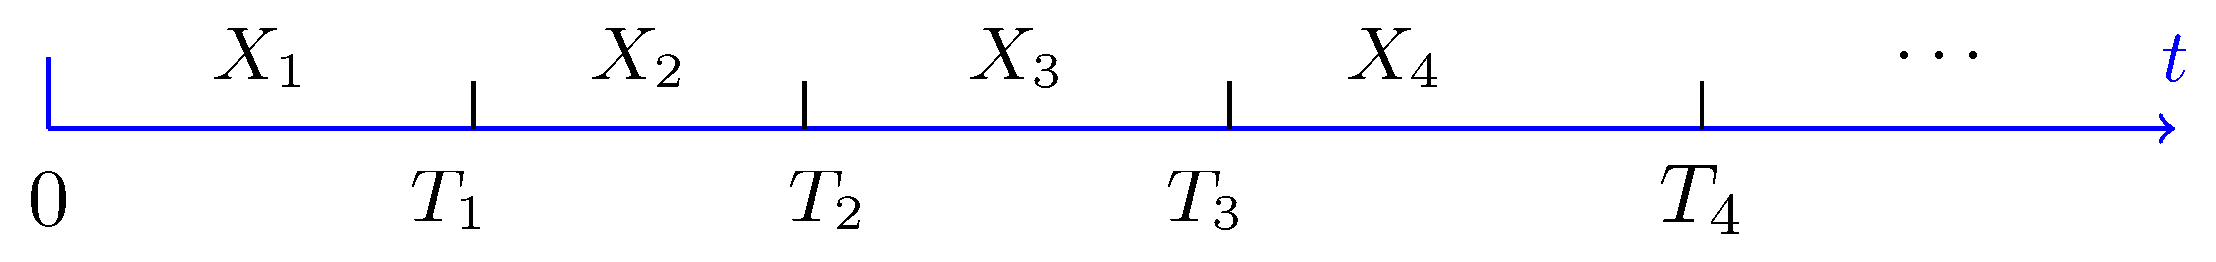
\includegraphics[height=1.5cm, width=13cm]{Poisson.png}$$

\begin{itemize}
    \item $N(t)$: The number of arrivals in $[0,t]$.
    \item $N(I)$: The number of arrivals in $I\subset [0,\infty)$.
\end{itemize}

Characterization
\begin{itemize}
    \item iid
    \item $N(b)-N(a)\sim $Poisson($\lmabda(b-a))$\\
    $N(s_1),\;N(s_2)-N(s_1),\ldots, N(s_n)-N(s_{n-1})$ are independent
\end{itemize}

\subsection{Thinning Property}
$N(t)$ is a Poisson process with rate $\lmabda$. We assign a type $Y_j \in \{1,2,,\ldots,l\}$ for the $j^{th}$ arrival. We assume that $Y_1,Y_2,\ldots,$ are $iid.$\\

Let $N_j(t)$ be the number of arrivals with type $J$ in $[0,t]$. Then $N_j$ is a Poisson process of rate $P_j\cdot d$. $N_1,N_2,\ldotsN_j$ are independent.

\subsubsection{Example}
Vehicles arrive at a roll both with a rate of $2/min$. The probability that a given vehicles is a truck is 2/3.
\begin{enumerate}[label=(\alph*)]
    \item P(exactly 2 cars and 3 trucks arriving in the next 5 minutes)
    \begin{itemize}
        \item Arriving vehicles form a Poisson process with rate $\lambda=2$.
        \item Let $N_1$ be the number of arrivals of trucks and $N_2$ be that of arrivals of cars.
        \item Then, for trucks, the rate of Poisson process is $\frac{2}{3}\lambda$ and the rate of Poisson process for cars is $\frac{1}{3}\lambda$.
        \item So $P(N_1(5)=3,\;N_2(5)=2)=P(N_1(5)=3)P(N_2(5)=2) = \frac{(\frac{20}{3})^3}{3!}e^{-\frac{20}{3}}\cdot \frac{(\frac{10}{3})^2}{2!}e^{-\frac{10}{3}}$

    \end{itemize}

    \item P(First arrival is a truck and the second one is a car) = $\frac{2}{3}\cdot \frac{1}{3}$
    \item Given that 20 trucks arrived in an hour what is expected the number of cars within the same hour? $\frac{1}{3}\cdot 60 = 20$\\
    
    The given 20 trucks actually does not affect the expected number of cars within the same time period.
\end{enumerate}

\subsection{Superposition Property}

Suppose that $N_1,\;N_2,\ldots,N_j$ are independent Poisson processes with the rate of $N_j$ is $\lambda_j$. We look at the union of all arrivals. This process is also a Poisson process, the rate $\lambda_1+\lambda_2+\ldots+\lambda_j$. The types of the arrivals will form an iid sequence where the probability of type $j = \frac{\lambda_j}{\lambda_1+\ldots+\lambda_j}$.

\vspace{1\baselineskip}
{\sl Proof.} Let $N_j$ be a counting functino of the $j^{th}$ Poisson process. Denote by $N$ the counting function of arrivals $N(t)=N_1(t)+N_2(t)+\ldots+N_j(t)$

$$N(b)-N(a)=\sum\limits_{j=1}^j \underbrace{(N_j(b)-N_j(a))}_{Poisson(\lambda_j(b-a))} \thicksim \text{ Poisson} \left((b-a)\sum\limits_{j=1}^k\lambda_j \right)$$


\subsubsection{Example}
Customers arrive at a ticket counter. 30 girls arrive per an hour and 20 boys arrive per an hour.
\begin{enumerate}[label=(\alph*)]
    \item What is the expected waiting time between the first and third customer?
    \begin{itemize}
        \item The arrival process of the customers is a Poisson process with rate 50/hour:\\
        Girls:$\frac{3}{5}$ Boys:$\frac{2}{5}$
        \item $\tau_1,\;\tau_2,\ldots \sim \exp(50)$\\
        $E[\tau_2+\tau_3] = E[\tau_2]+E[\tau_3] = \frac{1}{50}+\frac{1}{50} = \frac{1}{25}$
    \end{itemize}
    \item $P$(The first 3 customers are all )=$\left(\frac{3}{5}\right)^3$
\end{enumerate}

\subsection{Conditioning the Poisson Process}
We want to consider on $\{N(t)=k\}.$ What is the (conditional) distribution of the $k$ points in $[0,t)$.
\begin{itemize}
    \item $k=1$
    $$P(T_1\le s\;|\;N(t)=1) = \frac{P(T_1\le s)\capP(N(t)=1)}{P(n(t)=1)} = \frac{(P(N(s)=1)d,\;N(t)-N(s)=0)}{P(n(t)=1)} $$ $$=\frac{P(N(s)=1)P(N(t)-N(s)=0)}{P(N(t)=1)}
    =\frac{(\lambda s)e^{-\lambda s}\cdot e^{-\lambda(t-s)}}{(\lambda t)e^{-\lambda t}} = \frac{s}{t}$$
    
    $$
    P(T_1\le s\;|\;N(t)=1)= 
    \begin{cases}
        1 & \text{if } s \ge t\\
        \frac{s}{t} &  \text{if } 0< s < t\\
        0 & \text{if } s \le 0
    \end{cases}$$

\end{itemize}

{\bf Theorem} Let $\k\ge 1$. Then the conditional distribution of $(T_1,\;T_2,\ldots,T_k)$ given that $N(t) = k$

\newpage
{\bf Theorem 2.14} If we condition on $N(t) = n$, then the vector $(T_1,\;T_2,\ldots,\;T_n)$ has the same distribution as $(V_1,\; V_2,\ldots,\; V_n)$ and hence the set of arrival times $(T_1,\;T_2,\ldots,T_n)$ has the same distribution as $\{U_1,\;U_2,\ldots,U_n\}$\\
$$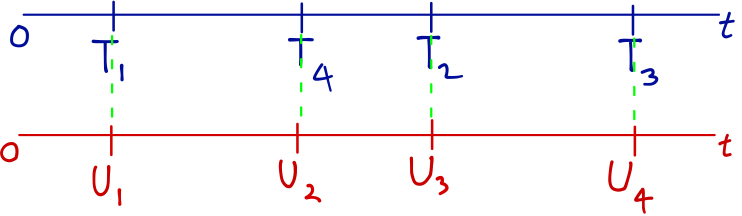
\includegraphics[height=1.5cm, width=11cm]{Thm_2_14.jpeg}$$
To construct the distribution $(T_1,\;T_2,\ldots,T_n)$ given $N(t)=n$
\begin{enumerate}[label=(\roman*)]
    \item Put on $[0,t]\; n\;i.i.d$ uniform random points $(U_1,U_2,\ldots,U_n)$
    \item Let $V_1<V_2<\ldots<V_n$ be the ordered set of values $(U_1,\ldots,U_n)$
    \item Then $(V_1,\ldots,V_n)$ has the same joint distribution as $(T_1,\;T_2,\ldots,T_n)$ \\ conditioned on $N(t)=n$
\end{enumerate}

Now $(T_1,\;T_2,\ldots,T_n)$ is the new distribution. Consequently, the joint PDF of $(T_1,\;T_2,\ldots,T_n)$ conditional on $N(t)=n$ is $f(x_1,\ldots,x_n)=\frac{n!}{t^n}$ on the set $\underbrace{\{0<x_1<x_2<\ldots<x_n<t\}}_{\text{These random variables are ordered}}$

\vspace{1\baselineskip}
{\sl Aside}
\begin{itemize}
    \item If $X$ is uniform $X\sim $Unif[a,b], then $X$ has PDF  
    $$f(x)=
    \begin{cases}
    \frac{1}{b-a}&x\in[a,b]\\
    0&x\notin[a,b]
    \end{cases}$$.
    \item $\vec{x} = (x_1,\ldots,x_n)$ is uniform on a set $H\subset \mathbb{R}^n$ if $\vec{x}$ has joint PDF $$f(x_1,\ldots,x_n)
    =\begin{cases}
    \frac{1}{VOL(H)}&(x_1,\ldots,x_n)\in H\\
    0&(x_1,\ldots,x_n)\notin H
    \end{cases}$$
    
The volume of uniform density on the set $\{0<x_1<x_2<\ldots<x_n<1\} = \frac{t^n}{n!}$ 

$$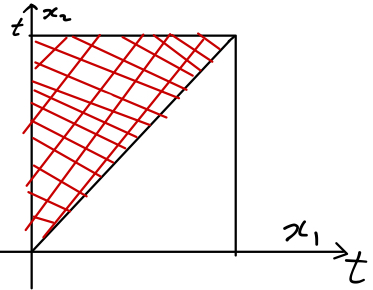
\includegraphics[height=3cm, width=4cm]{111.jpeg}$$
\newpage
{\sl Closer look at the case n=2}\\
If $X$ has CDF of $F$ and PDF of $f$, then $f(x)=F'(x)$.\\

Case $n=2:$ The joint CDF of $(X,Y)$ is $F(x,y)=p(X\le x,Y\le y)$. \\
If $(X,Y)$ has joint PDF $f$, then connection between 
$$F(x,y)=\int_{-\infty}^x\int_{-\infty}^y f(u,v)dvdu$$
If $f$ is continuous at $(x,y)$,
$$\frac{\partial^2}{\partial x\partial y} F(x,y)=f(x,y)$$

Let $U_1,U_2$ be independent uniform random variables on $[0,t]$. Let $V_1,V_2$ be $V_1=\min(U_1,U_2),\; \max(U_1,U_2)$. Find joint distribution function CDF $F_{V_1V_2}$ of ($V_1,V_2$). Let $u<v$.
$$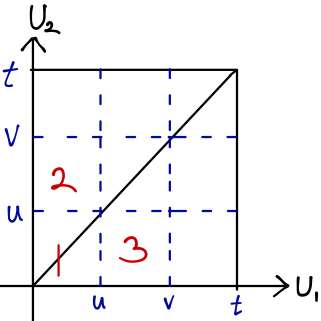
\includegraphics[height=3cm, width=4cm]{222.jpeg}$$
\begin{align}
    F(u,v) & = P(V_1\le u,\;V_2\le v) \nonumber \\
    &= P(U_1\le u,\;U_2\le U)+P(U_1\le u,\;u<U_2< v) + P(u<U_1\le v,\; U_2\le u) \nonumber \\
    & = \left(\frac{u}{t}\right)^2 + \left(\frac{u}{t}\right)\left(\frac{v-u}{t}\right)+
    \left(\frac{v-u}{t}\right)\left(\frac{u}{t}\right) = \frac{u^2+2uv-2u^2}{t^2} \nonumber
\end{align}
$$F_{V_1,V_2}(u,v)= \left(\frac{u}{v}\right)^2 + \frac{2u(v-u)}{t^2} \qquad \text{for } 0<u<v<t$$

\vspace{1\baselineskip}
Let $N(\cdot)$ be a rate $\lambda$ Poisson Process condition on $N(t)=2$. Find the conditional joint PDF. $(0\le u<v\le t)$
$$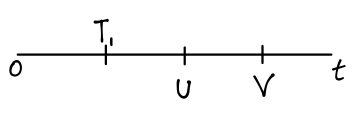
\includegraphics[height=1.3cm, width=6cm]{333.jpeg}$$
\begin{align}
    F_{T_1,T_2}(u,v\;|\;N(t)=2) & = P(T_1\le u,\; T_2\le v\;|\; N(t)=2)\nonumber \\ 
    &= P(N(u)\ge1\; N(v)=2\;|\; N(t)=2) \nonumber \\
    &= P(N(u) = 1,\; N(v)=2\;|\; N(t)=2) \nonumber \\
    &+ P(N(u)=2,\; N(v)=2\;|\; N(t) =2) \nonumber
\end{align}

$$=\frac{P(N(u)=1,\;N(v)=2,\;N(t)=2}{P(N(t)=2}+\frac{P(N(u)=2,\;N(v)=2,\;N(t)=2}{P(N(t)=2}$$
$$=\frac{P(N(u)=1,\;N(v)-N(u)=1,\;N(t)-N(v)=0)}{P(N(t)=2}+\frac{P(N(u)=2,\;N(v)-N(t)=2}{P(N(t)=2}$$

$$=\frac{e^{-u\lambda}u\lambda e^{-\lambda(v-u)}\lambda(v-u) e^{-\lambda(t-v)}+e^{-u\lambda}\frac{(u\lambda)^2}{2}e^{-\lambda(t-u)}}{e^{-t\lambda \cdot \frac{(-t\lambda)^2}{2}}}=\frac{2u(v-u)}{t^2}+\frac{u^2}{t^2} = \frac{2uv-u^2}{t^2}$$

Conditional Joint Density Function PDF 
$$f_{T_1,T_2}(u,v\;|\;N(t)=2) \frac{\partial^2}{\partial u \partial v}F_{T_1,T_2}(u,v\;|\;N(t)=2) = \frac{2}{t^2}$$

\vspace{2\baselineskip}
Find the conditional expectation: $E[T_n\;|\;N(t)=n]$\\

The conditional joint density function PDF $f_{T_n}(s\;|\;N(t)=n)=\frac{d}{ds} \left(\frac{s}{t}\right)^n = \frac{ns^{n-1}}{t^n}$ on the set $\{(x_1,\ldots,x_n)\;|\;0<x_1<\ldots<x_n<t\}$\\
$$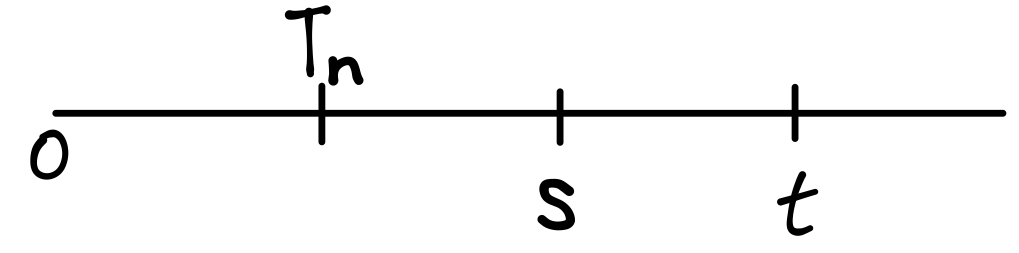
\includegraphics[height=1.3cm, width=6cm]{444.jpeg}$$

To find PDF of $T_n$, let's first find $P(T_n\le s\;|\;N(t)=n)=\left(\frac{s}{t}\right)^n$.
$$f_{T_n} (s\;|\;N(t)=n) = \frac{d}{ds}\left(\frac{s}{t}\right)^n = \frac{ns^{n-1}}{t^n}\qquad (0\le s \le t)$$
$$E[T_n\;|\;N(t)=n] = \int_0^t \frac{s\cdot ns^{n-1}}{t^n}ds = \frac{n}{n+1}t$$

P(arrivals at least u time units apart $|$ N(t)=2) = $\int_0^{t-a}\int_{x+a}^t \frac{2}{t^2}dydx = \frac{(t-a)^2}{t^2}$

$$\text{Probability}:\frac{\text{shaded area}}{t^2} = \frac{(t-u)^2\cdot \frac{1}{2}\cdot 2}{t^2}$$
$$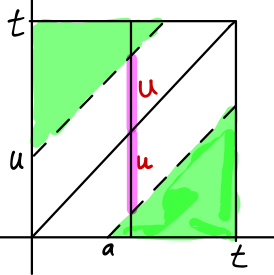
\includegraphics[height=4cm, width=5cm]{555.jpeg}$$
\end{itemize}

\subsection{Practice Exam}
{\bf 1.d} Let N be the proccess of ice cream cones sold with rate 3.
$$\text{$\lambda_c:$ Rate for chocolate= $0.7\cdot 3$}\quad
\text{$\lambda_s:$ Rate for strawberry = $0.2\cdot 3$}\quad
\text{$\lambda_v:$ Rate for vanilla= $0.1\cdot 3$}$$
\begin{itemize}[label={}]
   
    \begin{align}
        P(N_s(6,9]=2\;|\;N(7,9]=5)&= \frac{P(N_5(6,9]=2,\;N(7,9]=5)}{P(N(7,9]=5)}\nonumber \\
        &=\sum\limits_{j=0}^2\frac{P(N_s(6,7]=j,\;N_s(7,9)=2-j,\;N(7,9]=5)}{P(N(7,9]=5)} \nonumber \\
        &=\underbrace{\sum\limits_{j=0}^2\frac{P(N_s(6,7]=j)\overbrace{P(N_s(7,9]=2-j,\;N(7,0]=5)}^{\substack{P(N_s(7,9]=2-j,\; N_{cv}(7,9]=3+j):\\
        \text{Independece by the thinning property}}}}{P(N(7,9]=5)}}_{\text{Independence of arrivals in (6,7] \& (7,9]}} \nonumber \\
        &= \sum\limits_{j=0}^2
        \frac{e^{\frac{3}{5}}(\frac{3}{5})^j\cdot \frac{1}{j!}\cdot e^{-\frac{6}{5}}(\frac{6}{5})^{2-j}\frac{1}{(2-j)!}\cdot e^{-\frac{24}{5}}(\frac{24}{5})^{3+j}\frac{1}{(3+j)!}}
        {e^{-6}\frac{6^5}{5!}} \nonumber \\
        &= \sum\limits_{j=0}^2 \underbrace{e^{-\frac{3}{5}}\left(\frac{3}{5}\right)^j\frac{1}{j!}}_{\substack{\text{Poisson probability for}\\ \text{strawberries in (6,7]}}}
        \underbrace{\binom{5}{2-j}  \left(\frac{1}{5}\right)^{2-j}\left(\frac{4}{5}\right)^{3+j}}_{\substack{\text{Binomial probability of}\\ \text{  strawberries in (7,9],} \\ \text{comes from conditioning on} \\  \text{the total number of sales}}} \nonumber 
    \end{align}
\end{itemize}


\vspace{2\baselineskip}
{\bf Example: $P(T_3\le s\;|\;N(t)=4)$}
\begin{align}
    P(T_3\le s\;|\;N(t)=4)=P(N(s)\ge 3\;|\; N(t)=4) &=P(N(s)=3\;|\;N(t)=4)+P(N(s)=4\;|\;N(t)=4) \nonumber \\
    &=P(\text{out of 4 independent uniforms, 3 land in [0,5]}) \nonumber \\
    &+P(\text{out of 4 independent uniforms, all 4 land in [0,5]})\nonumber \\
    &=4\binom{s}{t}^3\left(1-\frac{s}{t}\right)+\left(\frac{s}{t}\right)^4 \nonumber
\end{align}

Longer way: $P(T_3\le s\;|\;N(t)=4)$
\begin{align}
    =\frac{P(N(s)=3,\;N(t)=4)}{P(N(t)=4)}+\frac{P(N(s)=4,\;N(t)=4)}{P(N(t)=4)} \nonumber \\
    =\frac{P(N(s)=3,\;N(s,t]=1)}{P(N(t)=4)}+
    \frac{P(N(s)=4,\;N(s,t]=0)}{P(N(t)=4)} \nonumber \\
    =\frac{e^{-s\lambda}(s\lambda)^3\frac{1}{3!}\cdot e^{-(t-s)\lambda}(t-s)\lambda}
    {e^{-t\lambda}(t\lambda)^4\frac{1}{4!}}
    +\frac{e^{-s\lambda}(s\lambda)^4\frac{1}{4!}\cdot e^{-(t-s)\lambda}(t-s)\lambda}
    {e^{-t\lambda}(t\lambda)^4\frac{1}{4!}} \nonumber \\
    &=\frac{4!}{3!}\frac{s^3(t-s)}{t^4}+\frac{s^4}{t^4} \nonumber
\end{align}

\vspace{2\baselineskip}
{\bf Fact}\\ 
Conditional on $N(t)=4,\; (T_1,\;T_2,\;T_3\;,T_4)$ has conditional PDF $f(x_1,\;x_2,\;x_3,\;x_4)=\frac{4!}{t^4}$ on the set $\underbrace{\{(x_1,\;x_2,\;x_3,\;x_4):\;0<x_1<x_2<x_3<x_4<t\}}_{\text{whose volume is }\frac{t^4}{4!}}$  
$$P(T_3\le s\;|\;N(t)=4) = \int\ldots\int \frac{4!}{t^4}dx_4dx_3dx_2dx_1 = \int_0^s dx_1\int_{x_1}^s dx_2\int_{x_2}^sdx_3\int_{x_3}^tdx_4 \frac{4!}{t^4}$$

\vspace{2\baselineskip}
{\bf 2.27} Person waits for a bus. Time till arrival of bus is Unif(0,1). Cars go by at rate 6. Each car gives this person a ride with probability 0.5. What is the probability that this person rides the bus.

\vspace{1.5\baselineskip}
{\sl Remark:} Arrivals come as a rate $\lambda$ Poisson process then interarrival times are Exp($\lambda$).
$$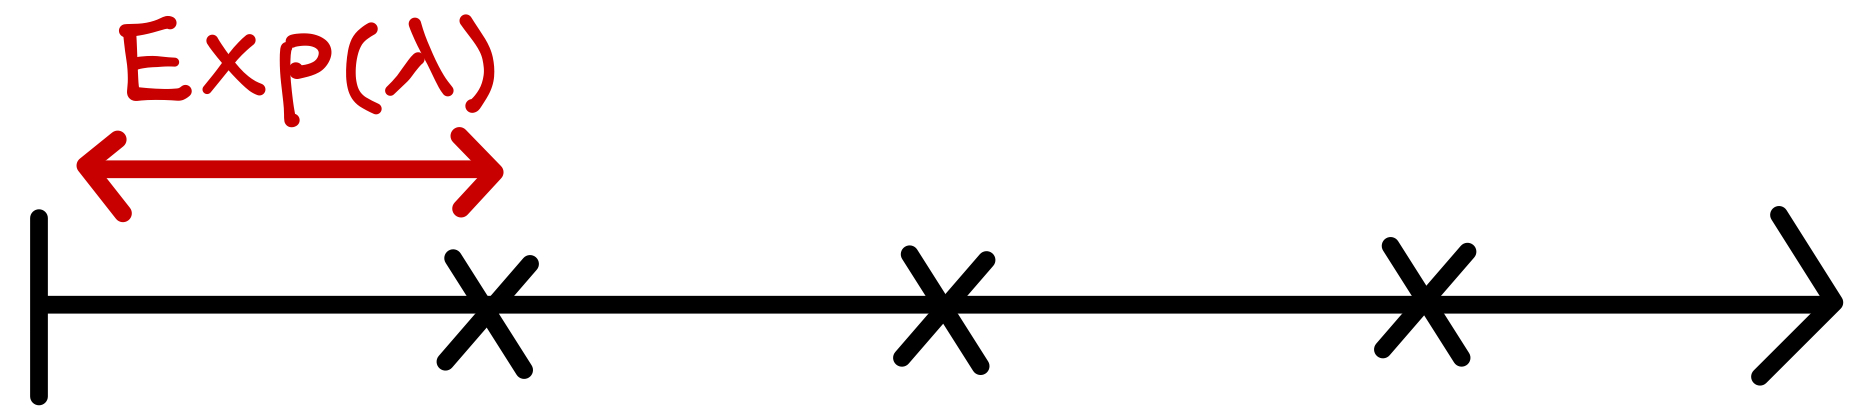
\includegraphics[height=1.2cm, width=8cm]{exp.jpeg}$$

\vspace{1\baselineskip}
$$
f_S(s)=
\begin{cases}
3e^{-3s}&s>0\\
0&s\le 0
\end{cases}
\qquad
f_U(s)=
\begin{cases}
1&s\in (0,1)\\
0&s\notin (0,1)
\end{cases}$$

\vspace{1\baselineskip}
\begin{align}
    P(U<S) &= \iint\limits_{u<s}\underbrace{f_U(u)f_S(s)duds}_{\text{Joint PDF of (U,S)}} \nonumber \\
    & =\int_0^1 1\; du\int_u^\infty 3e^{-3s}ds \nonumber \\
    &=\int_0^1 e^{-3u}du = \frac{1}{3}\int_0^1 3e^{-3u}du \nonumber \\
    &=\frac{1-e^{-3}}{3} \nonumber
\end{align}



$$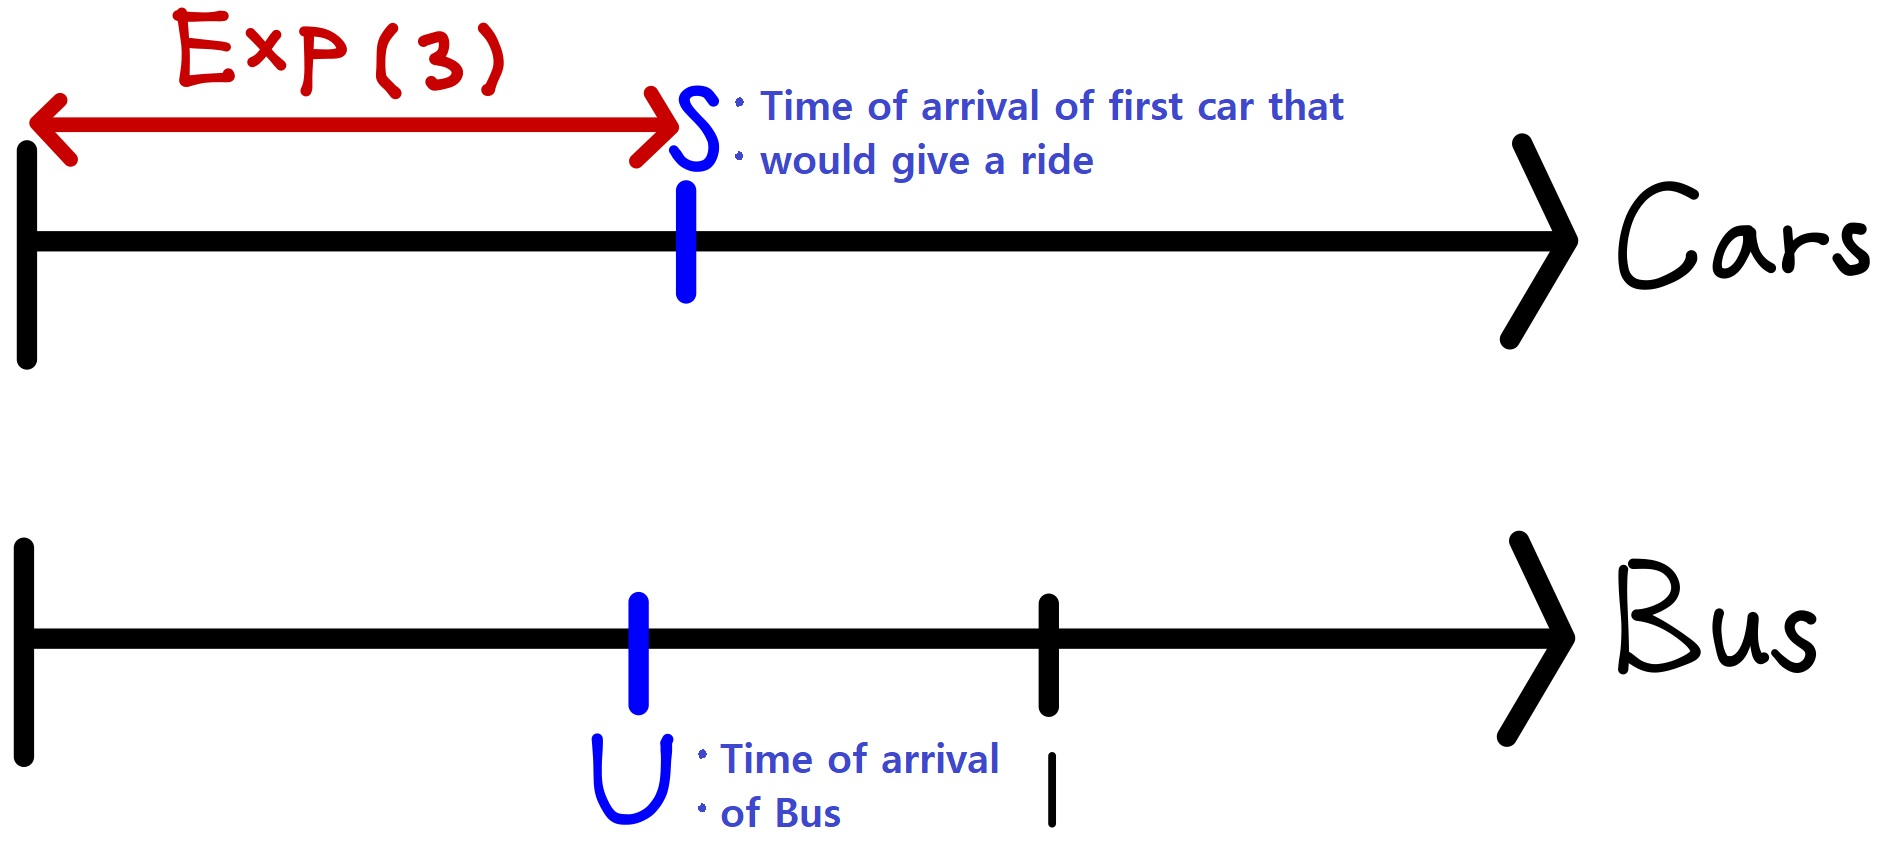
\includegraphics[height=4cm, width=10cm]{2_27.jpeg}$$

\end{section}
\end{document}
